\chapter{基于知识图谱的故障预测}
本章节主要介绍基于知识图谱的故障预测模型。在云计算场景中,分布式集群会随时间产生大量的事件序列。本文提出的故障预测模型可以利用已发生的事件序列,并结合知识图谱,预测是否会有故障产生以及具体产生何种故障,有助于运维人员提前检测、调整系统,防止故障真正发生而带来损失。具体实现上,该模型通过双向记忆网络获取实时事件序列编码表示,再使用上一章的表示学习模型获取知识图谱嵌入表示,最后将两者通过注意力权重计算相似度值,相似度值最高的知识图谱对应的故障信息即为所预测的故障。本模型在进行故障预测时取得了最高的准确率,且具有更高的细粒度与更好的可解释性。
\section{场景分析}
目前已经存在着较多相关的工作,但主要集中在研究数据的时序性。文献\parencite{pitakrat2018hora,zhang2018prefix,baldoni2015line}使用了统计学习和机器学习方法,如隐半马尔可夫模型(HSMM)、支持向量机(SVM)。然而,HSMM和SVM都建立于所有输入都是平稳且相互独立的假设之上,这种假设在云计算场景中是不成立的,因为云计算场景中不同组件产生的事件信息之间会存在一定的关联,比如先后时间顺序。为了处理时间序列数据进行故障预测,文献\parencite{xu2016health,cheng2018machine,du2017deeplog,das2018desh,islam2017predicting}使用深度学习方法如卷积神经网络(RNN)和长短期记忆神经网络(LSTM)进行预测。但RNN存在着难以克服的缺点,它会遗忘掉较远距离的数据信息。LSTM则克服了这个缺点,可以通过记忆门依然保留长距离数据的信息。文献\parencite{cheng2018machine,du2017deeplog,das2018desh}等工作已经使用LSTM在故障预测任务上比HSMM、SVM和RNN取得了更高的准确率。上述的方法都使用CPU使用率、内存使用率、未映射页缓存、平均磁盘I/O时间和磁盘使用率作为输入,把系统任务是否会失败作为输出。随后,文献\parencite{gao2020task}在LSTM的基础上使用了多层的Bi-LSTM、引入了任务优先级、提交时间、提交次数等更多的特征,还根据不同数据对故障的重要性赋予其不同的权重。

在本文场景中进行故障预测时,还需要考虑以下场景特性:

1)数据形式为事件序列。本文所有的数据,除了包括上文提到的CPU使用率、内存使用率、未映射页缓存、平均磁盘I/O时间和磁盘使用率,另外还有新引入的微服务启动、重启、程序运行日志等数据,都已经被转为统一规范化的事件数据,所以要处理的数据为事件序列。

2)需要引入知识图谱增强可解释性。本文在进行故障预测时,已经存在了前文所构建的组件-事件知识图谱,所以需要引入知识图谱进行故障预测,这样会使预测结果更具可解释性,还能具体到会预测出现何种故障,而之前的工作只能预测有无故障。
\begin{figure}[htbp]
    \centering
    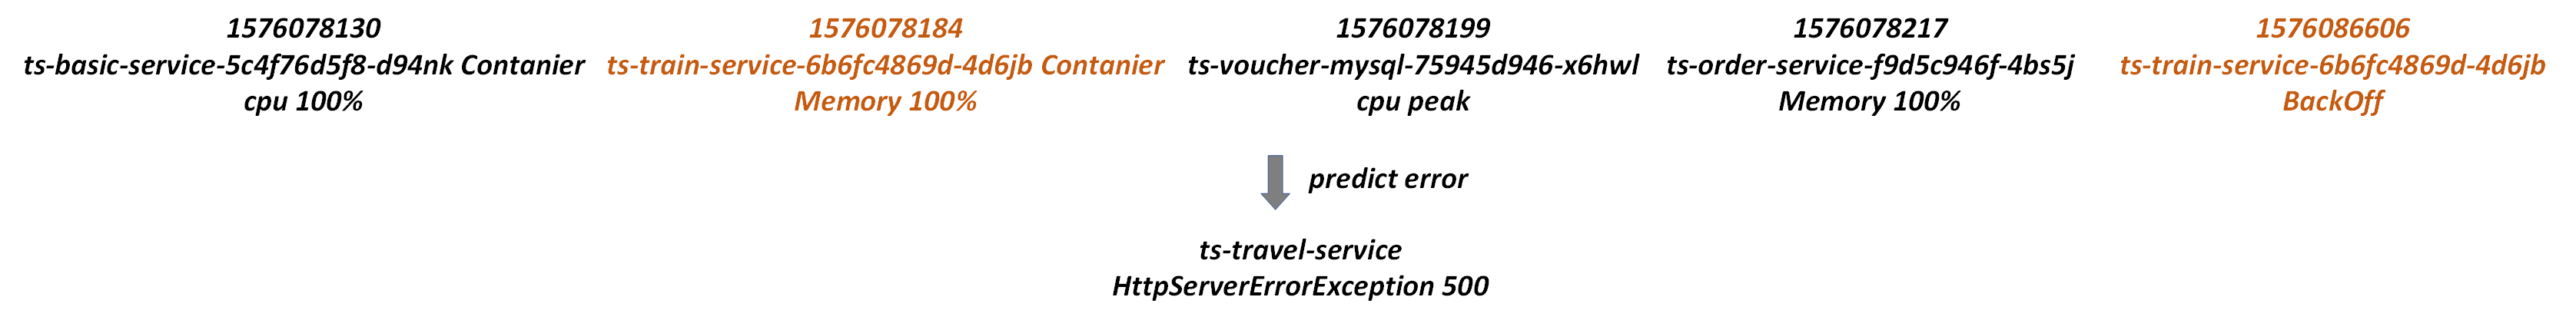
\includegraphics[width=1.0\textwidth]{predict-case.png}
    \caption{事件序列故障预测\label{predict-case}}
\end{figure}

3)事件权重分配需要考虑事件所在的上下文,不能仅根据数据对故障的重要性赋予权重。如图\ref{predict-case}所示是一个实时事件序列案例。在进行故障预测时,并不是每个异常事件都是同等重要的。$ts-train-service-6b6fc4869d-4d6jb$上的$Contanier Memory 100\%$和$ts-train-service-6b6fc4869d-4d6jb$上的$BackOff$事件应当比其他事件的重要性更高,因为这两个事件的发生意味着$ts-train-service$所在的$Container$已经内存不足,使得$ts-train-service$微服务无法正常启动,后续导致$ts-travel-service$发生$  HttpServerErrorException 500$的可能性极高。而其它的事件如$ts-order-service-f9d5c946f-4bs5j$上的$Memory 100\%$虽然对图\ref{order-service-error}的“订票服务不可用”故障较为重要,但是并没有发生后续的关键事件类型$ts-order-service backoff$,所以其重要性较低。

基于以上的分析,本文在编码事件序列时,依然选择基于LSTM的模型,但不同于之前根据每个事件元素对故障重要程度赋予权重\cite{gao2020task},本文选择使用组件-事件知识图谱的嵌入向量来对各个时间单元的数据计算注意力权重,即由组件-事件知识图谱选取其所关注的信息。

\section{基于记忆网络的故障预测算法}\label{memory-net-section}
本小节主要介绍了文献\parencite{gao2020task}在进行故障预测时所使用的记忆神经网络。
\subsection{模型结构}
\begin{figure}[htbp]
    \centering
    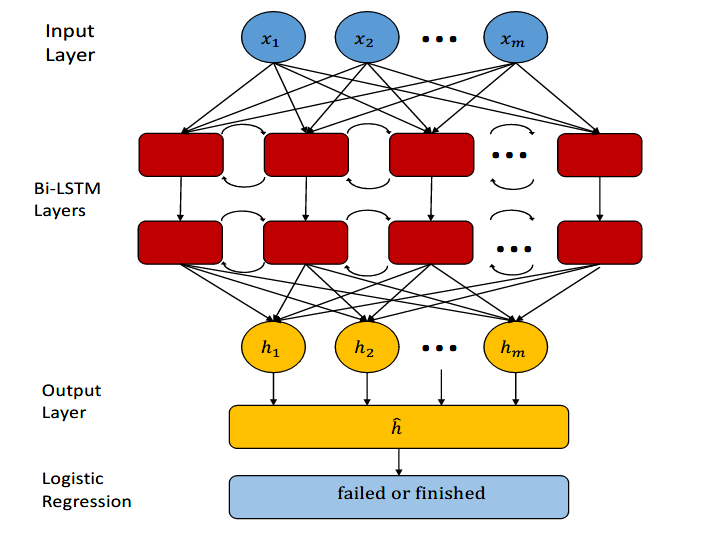
\includegraphics[width=.7\textwidth]{bilstm-model.png}
    \caption{双向记忆网络\label{bilstm-model}}
\end{figure}
图\ref{bilstm-model}所示为双向记忆神经网络,可见其包含输入层、两层Bi-LSTM、输出层和逻辑回归层。

输入层主要是数据的嵌入层。文献\parencite{gao2020task}拼接了同一时间点的CPU使用率、内存使用率、未映射页缓存、平均磁盘I/O时间、磁盘使用率、任务优先级、提交时间和提交次数共计8个特征。这样之后每个时间点都是一个8维的嵌入向量。
\begin{figure}[htbp]
    \centering
    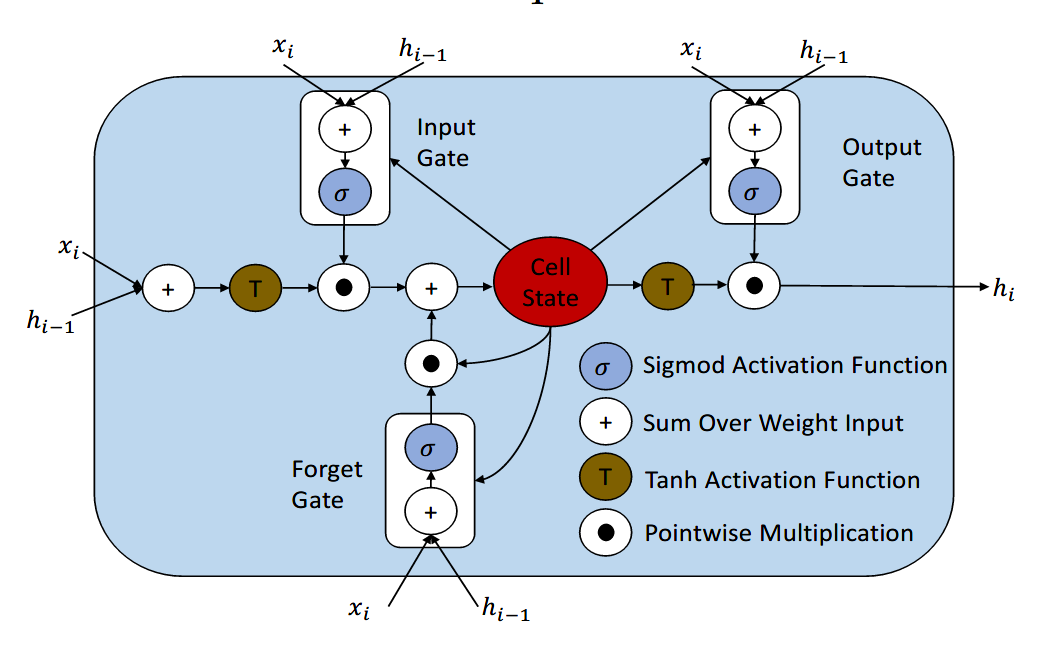
\includegraphics[width=.7\textwidth]{lstm-cell.png}
    \caption{记忆网络单元\label{lstm-cell}}
\end{figure}

Bi-LSTM层完成了对时序数据的特征编码。该层会将输入的时序数据分别进行前向编码和后向编码,再将得到的前向隐状态和后向隐状态拼接得到最终的隐状态。经过上述步骤后,每个时间点的隐状态都会得到正向反向的上下文信息。图\ref{lstm-cell}展示了LSTM神经元内部的结构,可见其主要利用了非线性函数选择数据保存还是舍弃。具体实现上,每个神经元内部共有三个门控制其状态,包括输入门、遗忘门和输出门。输入门决定了应该更新哪个神经元状态,遗忘门决定了应该忽视掉什么信息,输出门决定输出隐状态的哪部分信息。该过程可以用公式\ref{lstm-cell-equation}表示:
\begin{equation}
    \begin{array}{l}
    g_{i}=\varphi\left(w_{g x} x_{i}+w_{g h} h_{i - 1}+b_{g}\right) \\
    n_{i}=\sigma\left(w_{n x} x_{i}+w_{n h} h_{i- 1}+b_{n}\right) \\
    f_{i}=\sigma\left(w_{f x} x_{i}+w_{f h} h_{i- 1}+b_{f}\right) \\
    o_{i}=\sigma\left(w_{o x} x_{i}+w_{o h} h_{i- 1}+b_{o}\right) \\
    s_{i}=g_{i} \odot n_{i}+s_{i -1} \odot f_{i} \\
    h_{i}=\varphi\left(s_{i}\right) \odot o_{i}
    \end{array}
    \label{lstm-cell-equation}
\end{equation}
其中$w_{gx}, w_{nx}, w_{fx} $和$w_{ox} $是记忆单元输入$x_{i}$的权重系数。$w_{gh}, w_{nh}, w_{fh} $和$w_{oh} $是记忆单元上一步输出$h_{i}-1$的权重系数。$b_{g}, b_{n}, b_{f},$ 和 $b_{o}$分别为输入信息$g_{i}$、输入门$n_{i}$、遗忘门$f_{i}$和输出门$o_{i}$对应的偏置系数。而$s_{i}$和$s_{i-1}$则分别为时间$i$和$i-1$的神经元状态。另外,$\odot$代表点乘,$\sigma$代表sigmoid激活函数,$\varphi$代表tanh激活函数。

输出层目的在于将输入序列中每个记忆单元隐状态整合起来。具体方式是将输入$X=\left\{x_{1}, x_{2} \ldots x_{m}\right\}$传入Bi-LSTM得到的表示序列$\left\{h_{1}, h_{2} \ldots h_{m}\right\}$进行式\ref{mean-pool}中所示的平均池化操作,得到序列表示向量$\widehat{h}$。
\begin{equation}
    \widehat{h}=\frac{1}{m} \sum_{i=1}^{m} h_{i}
    \label{mean-pool}
\end{equation}

逻辑回归层是预测当前数据序列将来是否会有故障的二分类器。具体实现上,该层将输出层得到的向量表示$\widehat{h}$输入$\operatorname{logstic}(.)$函数,计算会出现故障的概率。当概率大于阈值时,则预测会出现故障;反之,则预测不会出现故障。

\subsection{模型训练}
基于记忆网络的故障预测模型的最终训练目标为正确分类每种数据序列。对应的损失函数为式\ref{memroy-net-loss}中所示。
\begin{equation}
    \mathcal{L}=-\sum_{i=1}^{n}\left[Y_{i} \log \left(f\left(X_{i} \right)\right)+\left(1-Y_{i}\right) \log \left(1-f\left(X_{i} \right)\right)\right]
    \label{memroy-net-loss}
\end{equation}
其中$X_{i}$表示第$i$条输入序列,$Y_{i}$为$X_{i}$对应的标签,即下一个时间点是否会有故障发生(1代表有故障发生,0代表不会有故障发生)。$f\left(.\right)$表示上文的网络模型。
\section{基于记忆网路和知识图谱的故障预测模型}
本小节主要介绍基于双向记忆网络和组件-事件知识图谱的故障预测模型。在上节已经介绍了编码时序数据的双向记忆网络,本节会进一步引入组件-事件知识图谱辅助故障预测,旨在提高故障预测的细粒度(预测到会出现何种故障)和预测结果可解释性。

\subsection{模型结构}
\begin{figure}[htbp]
    \centering
    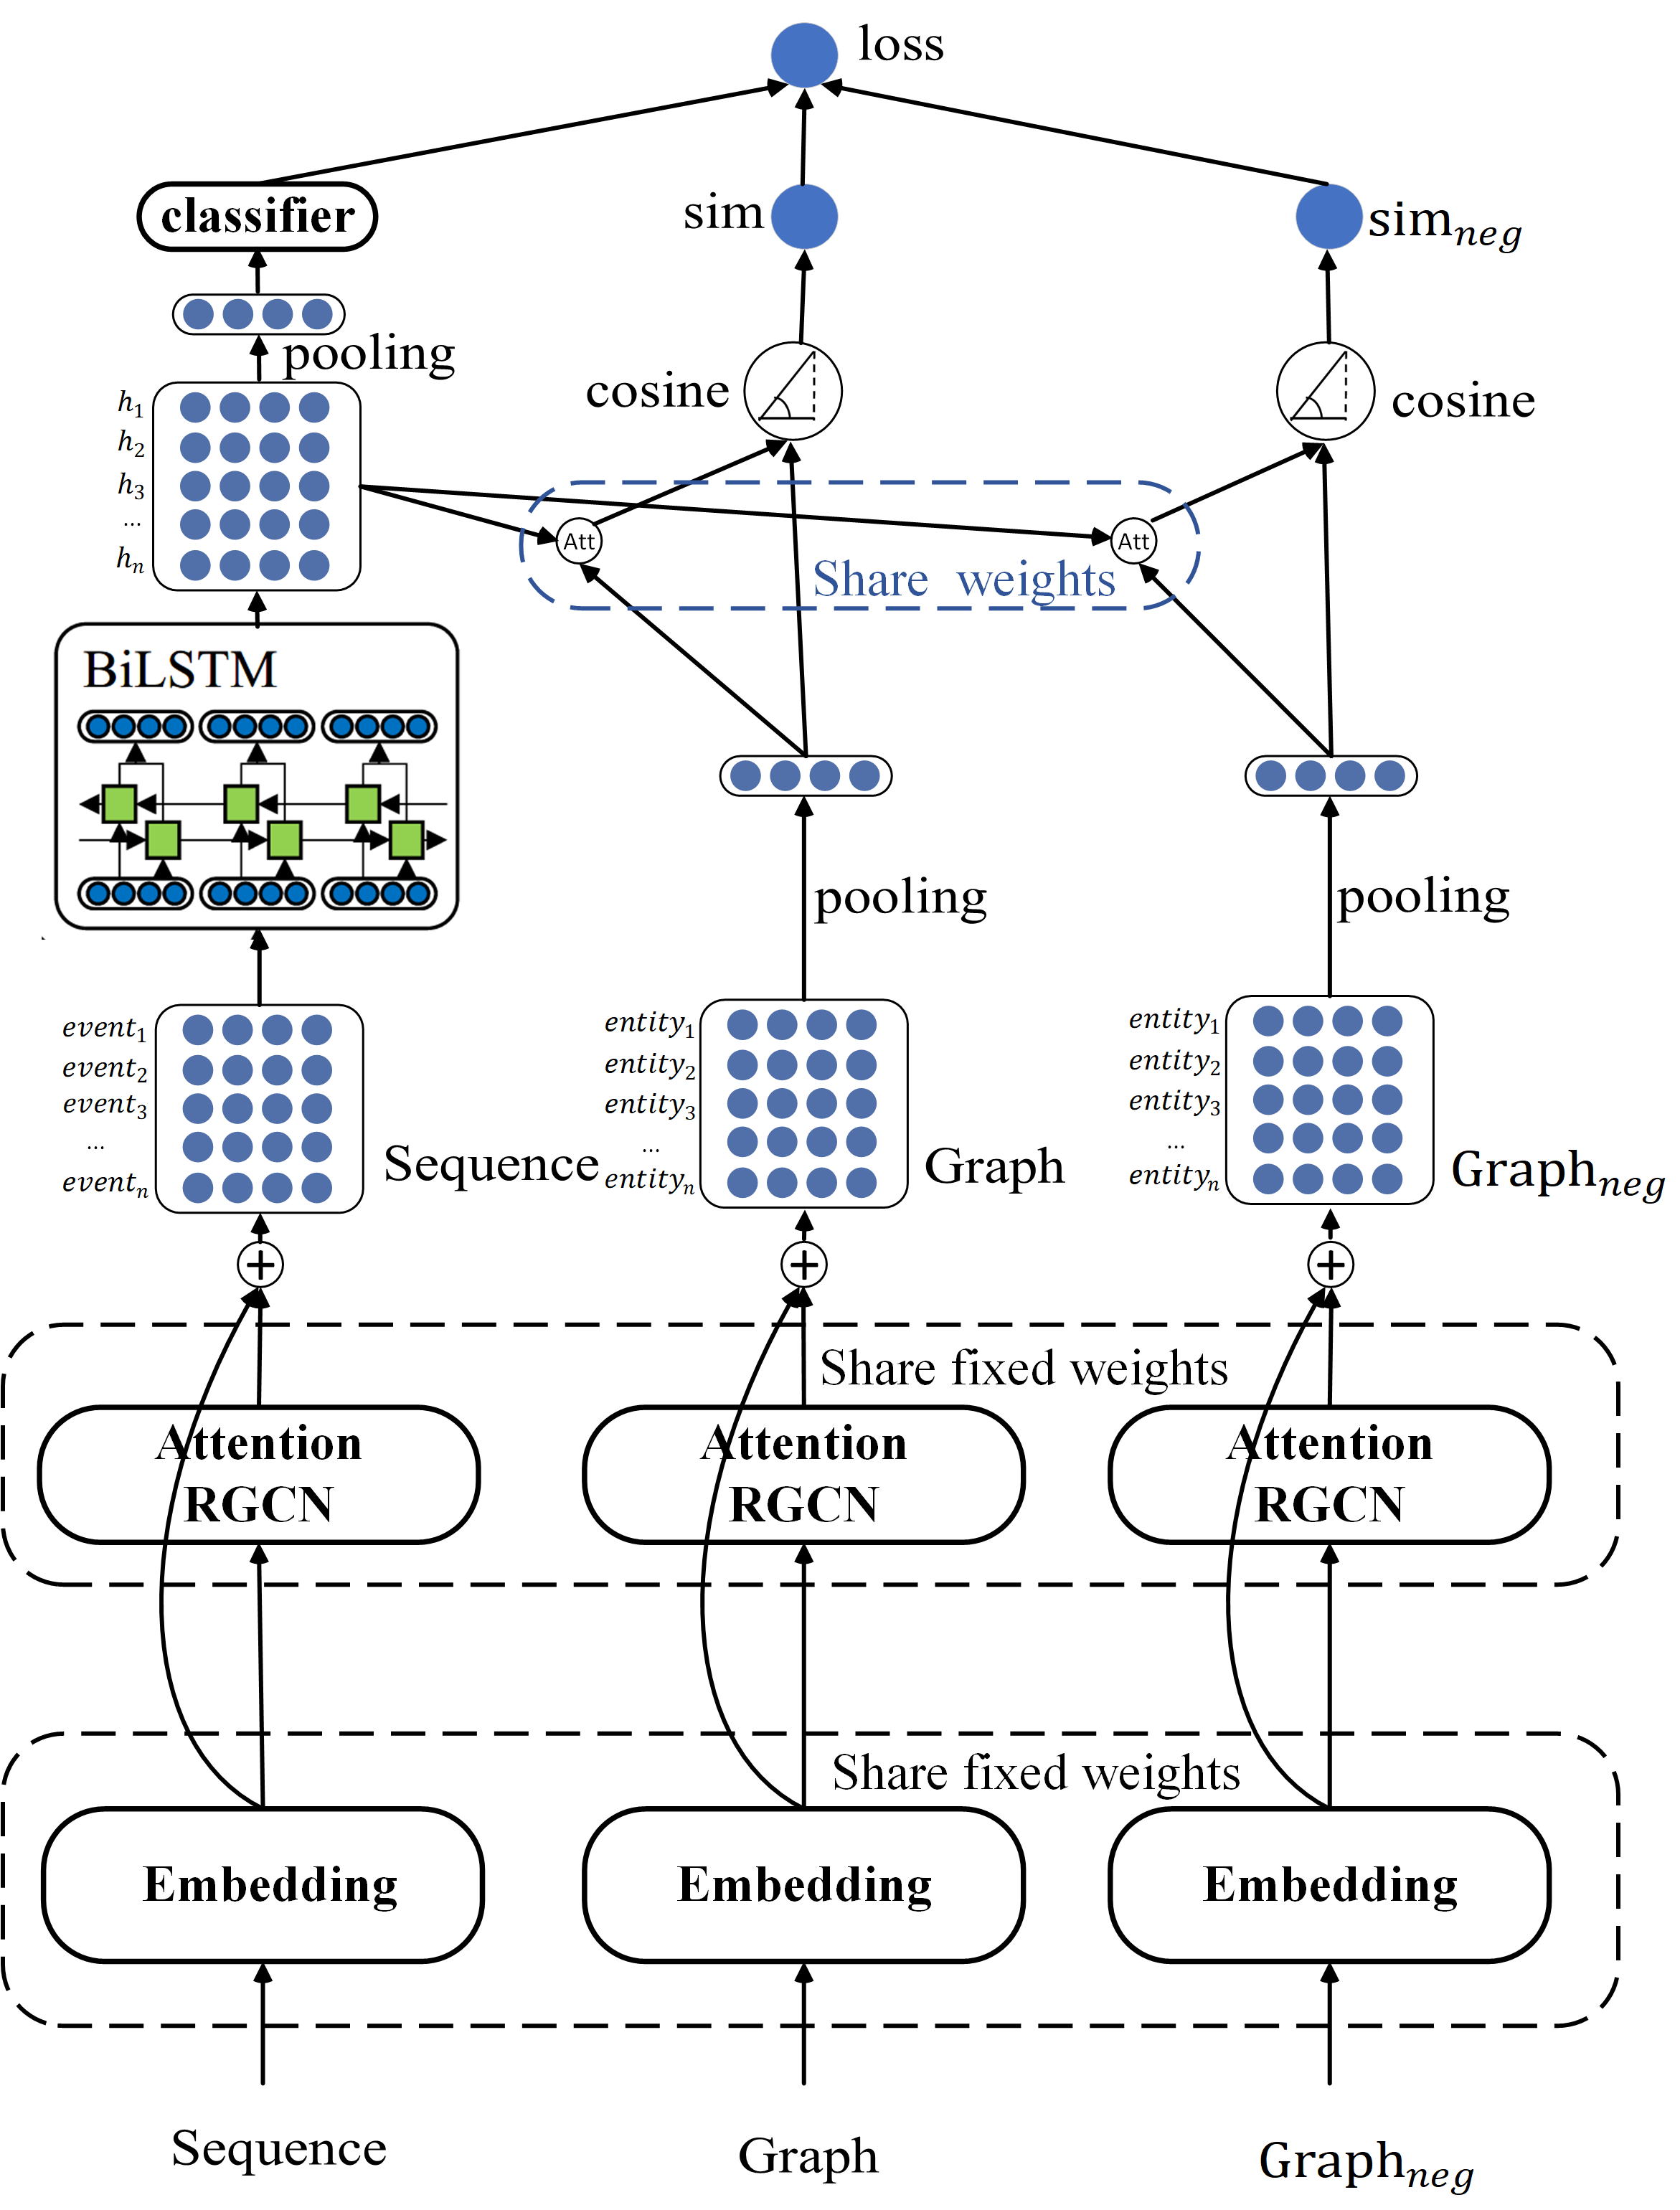
\includegraphics[width=.6\textwidth]{predict-error-model.png}
    \caption{故障预测模型\label{predict-error-model}}
\end{figure}
图\ref{predict-error-model}是引入组件-事件知识图谱的故障预测模型。其中嵌入层、Attention-RGCN使用组件-事件知识图谱表示学习模型的结构与参数,并固定不变。双向记忆网络使用上一小节的模型,参数后续进行训练学习。注意力层和分类层的参数也会在后续进行学习。

嵌入层规定了实时事件序列和知识图谱的嵌入方式。图\ref{input-event-sequence}为一个实时事件序列案例,可见实时事件序列中每个事件也都对应着所在的组件,且组件之间存在着拓扑关系,只是每个组件都有其唯一标识,但对应的组件类型未发生改变,所以同样可以使用图\ref{kg-representation}中的表示学习模型,获取每个实时事件的嵌入表示向量。组件-事件知识图谱则同图\ref{graph-example}所示。输入层中的embedding和Attention-RGCN均使用章节\ref{representation-paras-learn}所学到的参数并固定,实时事件序列和组件-事件知识图谱都会共享这些参数用于嵌入表示。
\begin{figure}[htbp]
    \centering
    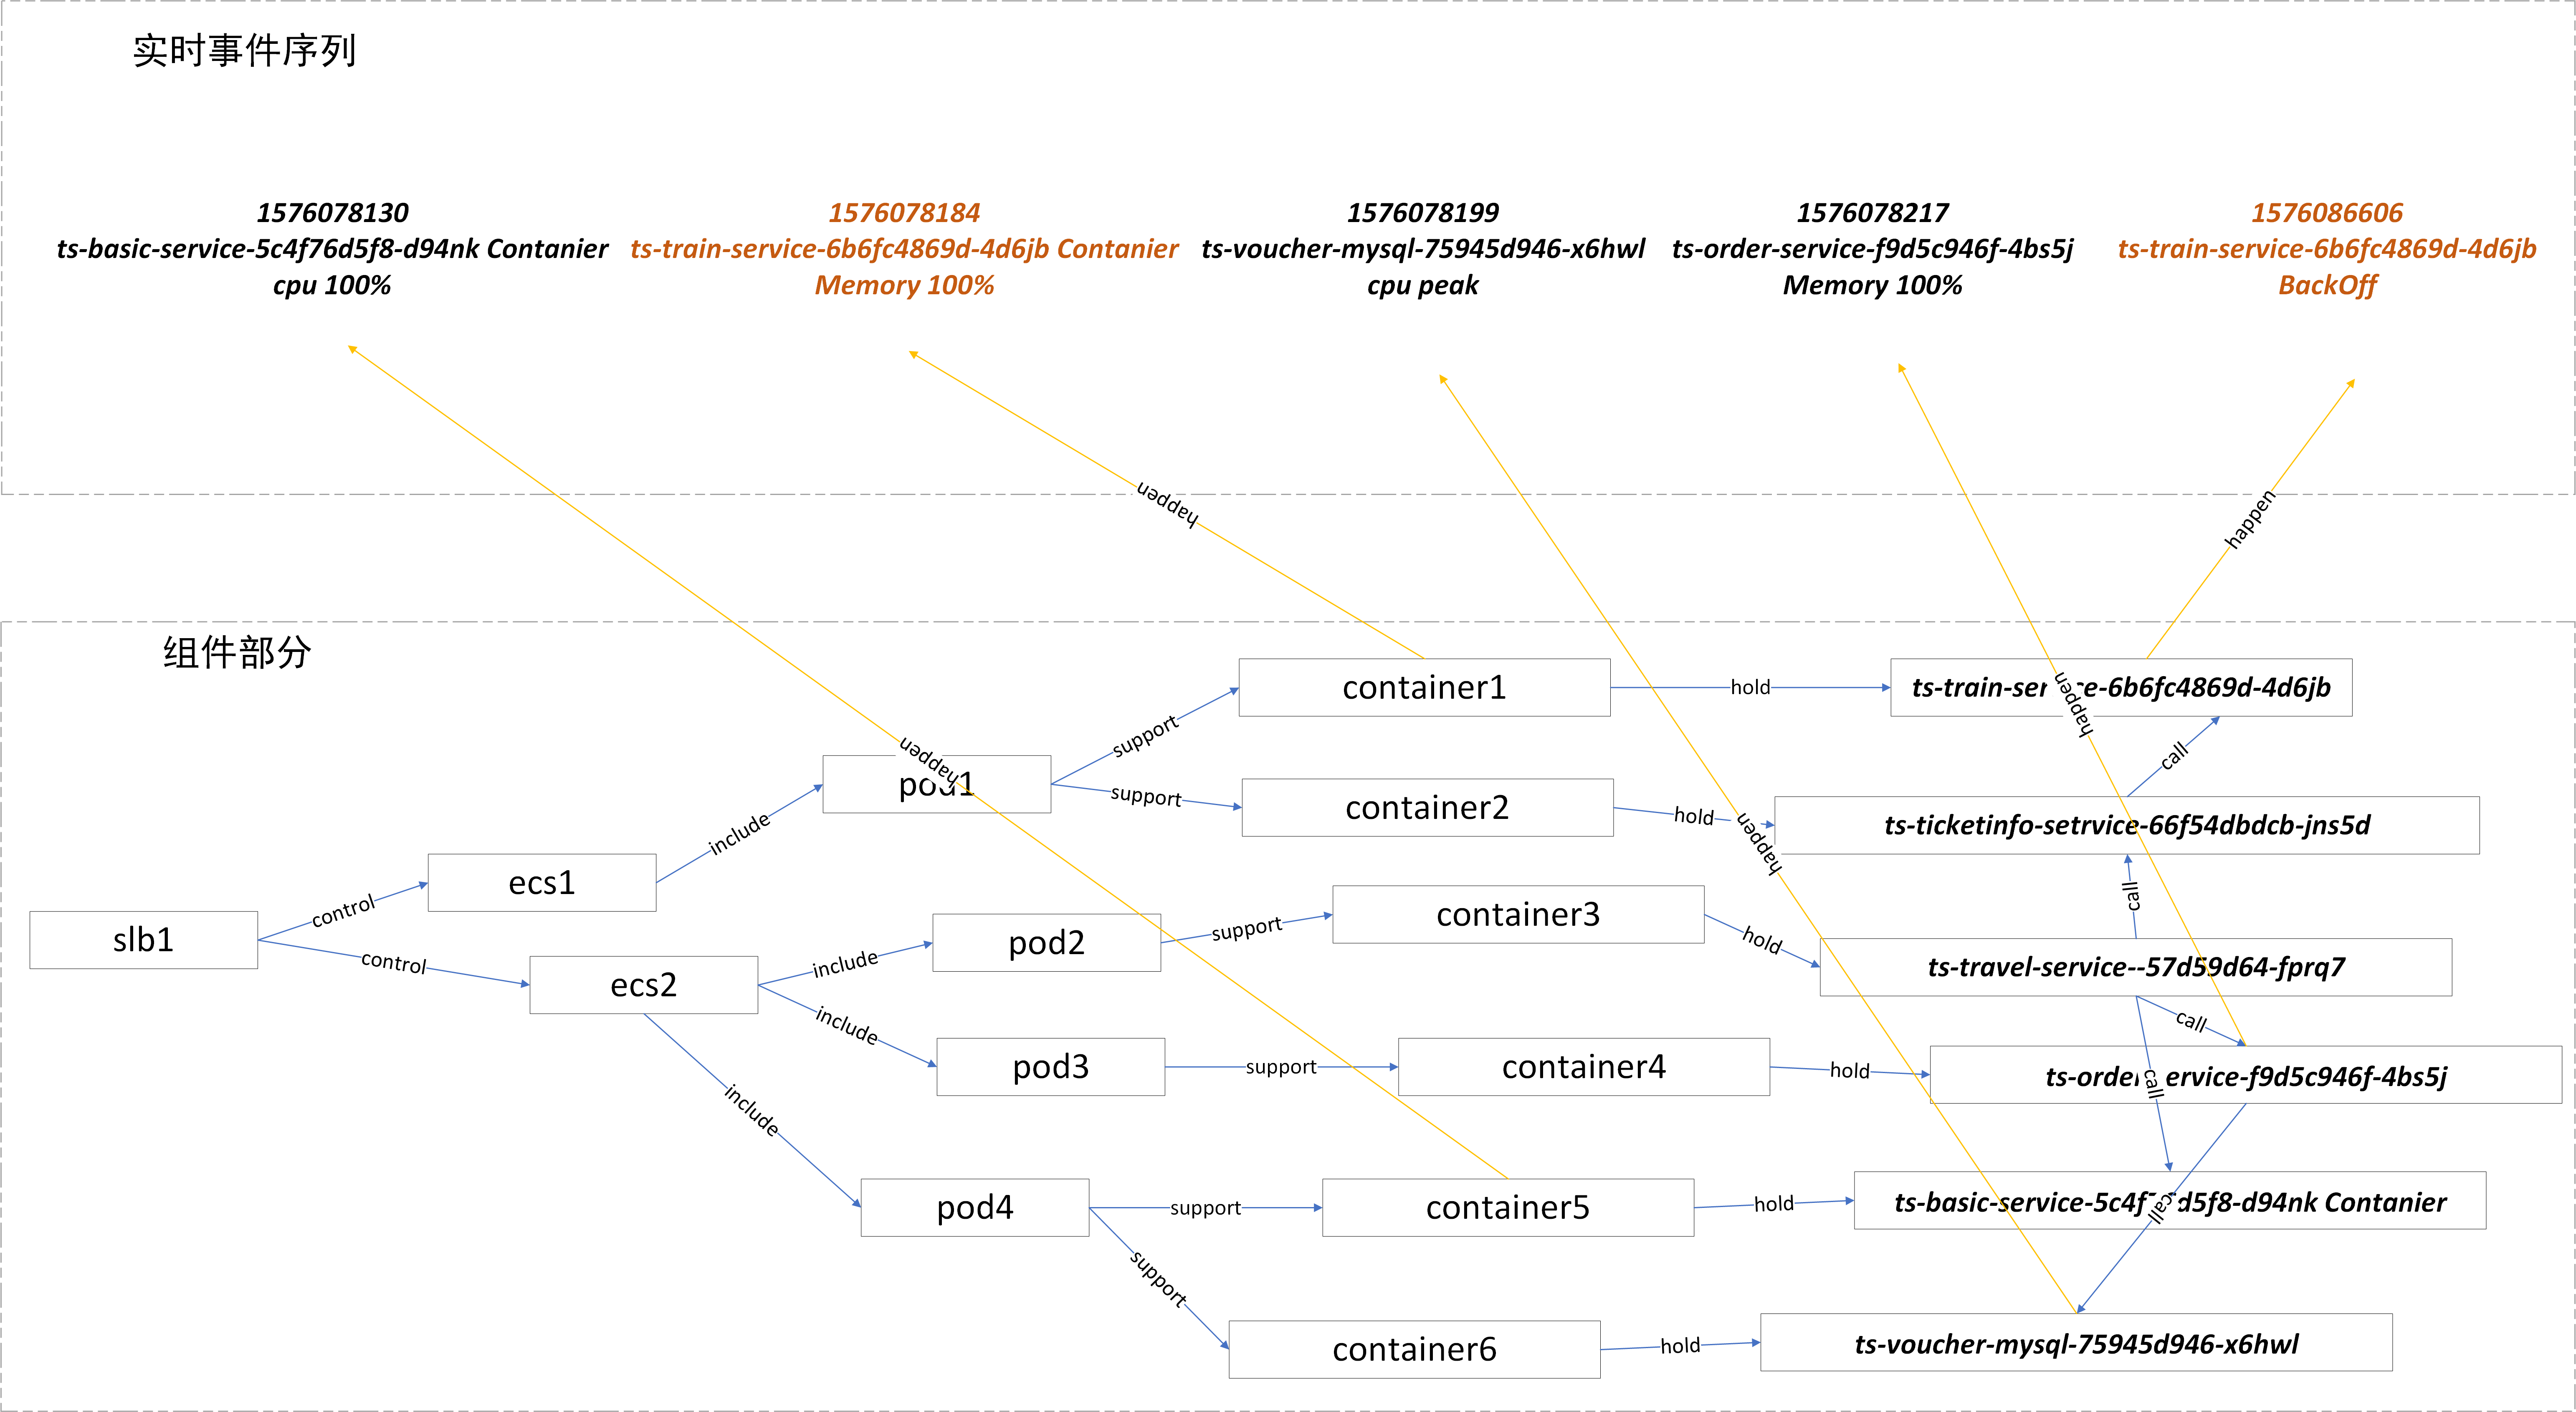
\includegraphics[width=.9\textwidth]{input-event-sequence.png}
    \caption{输入实时事件序列样例\label{input-event-sequence}}
\end{figure}

双向记忆网络层用来获取实时事件序列之间的时序特征。在实时事件序列中,虽然存在着组件之间的拓扑关系,但不存在事件之间的因果关系,事件之间只存在着前后的时序信息。记忆网络层使用上节\ref{memory-net-section}中的双向记忆网络模型,该模型已经在已有的故障预测工作中取得了最佳的效果。

在注意力层中,特定故障类型的组件-事件知识图谱会对经过双向记忆网络得到的隐状态序列做注意力权重累加。这样的注意力计算方式可以让知识图谱选择其所关注的事件子序列,并减少了噪声事件的干扰。输入事件序列$X=\left\{x_{1}, x_{2} \ldots x_{m}\right\}$在经过嵌入层和双向记忆网络后会得到隐向量序列$\left\{h_{1}, h_{2} \ldots h_{m}\right\}$。如式\ref{sequence-hidden}所示,注意层会首先计算知识图谱对隐状态序列的权重$\alpha_{(. , g)}$,然后进行权重累加获取事件序列嵌入表示$h_{sequence}$。

\begin{equation}
    \begin{array}{l}
    e_{(h_{i} , g)} = h_{i}\mathbf{W}g\\
    \alpha_{(h_{i} , g)}=\operatorname{softmax}\left(e_{(h_{i} , g)}\right)=\frac{\exp \left(e_{(h_{i} , g)}\right)}{\sum_{j=0}^{m}  \exp \left(e_{\left(h_{j} , g\right )}\right)}\\
    h_{sequence} = \sum_{i=0}^{m}\alpha_{(h_{i} , g)}\cdot h_{i}\\
    \end{array}
    \label{sequence-hidden}
\end{equation}

输出层分为两方面,一方面会将双向记忆网络的输出平均池化后得到的向量直接进行预测分类(有无故障),另一方面将组件-事件知识图谱的嵌入表示与注意力层权重累加得到的序列嵌入表示$h_{sequence}$做相似度计算,输出每张故障类型对应组件-事件知识图谱的相似度得分,按得分从高至低排列,即可得到预测故障类型排列结果。

\subsection{参数学习}
模型的损失函数如式\ref{graph-sequence-predict}所示,分为两部分。在预测判别有无故障时,使用基于交叉熵的损失函数。在知识图谱相似匹配时,通过负采样用边际损失作为损失函数。
\begin{equation}
    \begin{aligned}
        \mathcal{L}=-\sum_{i=1}^{n}[Y_{i} \log \left(f\left(X_{i} \right)\right)
        +\left(1-Y_{i}\right) \log \left(1-f\left(X_{i} \right)\right)\\
+Y_{i}\cdot \max \left (0, \cos \left (h_{i}, g_{neg} \right ) - \cos \left (h_{i}, g \right )\right )]
    \end{aligned}
    \label{graph-sequence-predict}
\end{equation}

其中,$X_{i}$为第$i$个输入事件序列$\left\{x_{1}, x_{2} \ldots x_{m}\right\}$,$Y_{i}$为第$i$个输入事件序列有无故障的标签(0表示输入事件序列无故障,1表示输入事件序列有故障)。$h_{i}$为$X_{i}$事件序列的隐状态嵌入表示,$g$为$X_{i}$对应故障类型的组件-事件知识图谱的嵌入表示,$g_{neg}$为负采样任意一个与$X_{i}$不匹配的组件-事件知识图谱的嵌入表示向量。

\section{本章小结}
本章主要介绍了基于实时事件序列和组件-事件知识图谱的故障预测,通过上一章的组件-事件知识图谱表示学习模型获取每个故障类型对应的组件-事件知识图谱的嵌入表示向量,然后对双向记忆网络编码的实时事件序列隐状态进行注意力权重累加获取事件序列嵌入表示,最后计算两个嵌入表示向量的相似度,按照相似度从高至低排序即可得到预测的故障类型列表。本文的故障预测模型可以具体到故障类型,同时引入组件-事件知识图谱进行注意力计算,使得预测结果具有了可解释性。